\documentclass{beamer}
%%%%%%%%%%%%%%%%%%%%%%%%%%%%%%%  Packages  %%%%%%%%%%%%%
\usepackage{amsmath} 
\usepackage{mathtools}
\usepackage{physics}
\usepackage{amssymb}
\usepackage{mathptmx}
\usepackage{array}
  
%%%%%%%%% FIGurES %%%%%%%%%%%%%%%%%%%%%%%%
\usepackage{textcomp}
\usepackage{graphicx}
\usepackage{caption} 
\usepackage{subcaption}
\usepackage{scrextend}
\usepackage{rotating}
\usepackage{float}
\usepackage{hyperref}

%\usepackage[loop,controls,buttonsize=0.24cm,buttonbg=0.8,autoplay]{animate}
\usepackage{multimedia}
%\usepackage{xmpmulti}

%\usepackage{media9}

%\graphicspath{{./figures/}}
\hypersetup{colorlinks=true, citecolor=blue, linkcolor=blue}
\renewcommand{\equationautorefname}{Eq.}
\renewcommand{\figureautorefname}{Fig.}
 
%%%%%%%%%%%% LaNgUaGe %%%%%%%%%%%%%%%%%%
\usepackage{verbatim}
\usepackage{natbib}
\usepackage{wrapfig}
\usepackage[utf8]{inputenc}

%%%%%%%%%%%%%% PhYsIcS %%%%%%%%%%%%%%%%%%%%%%%

\renewcommand{\annia}{\hat{a}}
\renewcommand{\annib}{\hat{b}}
\renewcommand{\creata}{\hat{a}^\dagger}
\renewcommand{\creatb}{\hat{b}^\dagger}

\renewcommand{\a}{a^ }
\renewcommand{\b}{b^ }
\renewcommand{\adag}{a^\dagger}
\renewcommand{\bdag}{b^\dagger}

\usepackage{qcircuit}

\usetheme{PaloAlto}

\title{Modelling Nonlinear optics with the Bloch-Messiah reduction}
\author{Oliver Thomas}
\institute{Quantum Engineering CDT \\ University of Bristol}
\date{\today}

% plan

\begin{document}

% slide 1
\frame{\titlepage}

% slide 2
\begin{frame}
\frametitle{Overview}
\begin{itemize}
	\item What is nonlinear optics?
    \item Why do we care about it?
    \item What I have been doing
    \item Gaussian optics 
    \item Outlook
\end{itemize}
\end{frame}

%slide 3
\begin{frame}
\frametitle{Motivation}
\begin{columns}
\column{0.5\textwidth}
    \begin{block}{The good}
    Spontaneous Parametric processes, SPDC, SFWM
    \begin{itemize}
        \item Heralded single photon sources
        \item Entangled photon pair generation (polarisation, spatial)
    \end{itemize}
    Kerr processes 
    \begin{itemize}
        \item Self-Phase modulation (SPM) for generating Bannana states (CV)
        \item Cross-Phase modulation (XPM) for sensing
    \end{itemize}
    \end{block}
%
\column{0.5\textwidth}
    \begin{block}{The bad}
        \begin{itemize}
            \item Generating more than two photons -$>$ bad for quantum computing
        \end{itemize}
        All Kerr nonlinear processes 
        \begin{itemize}
            \item SPM -$>$ Spectral broadening
            \item XPM -$>$ Unwanted phase shifts on single photons due to propagation of the pump 
        \end{itemize}
        \end{block}
\end{columns}

\end{frame}

% slide 4
\begin{frame}
\frametitle{What do we mean by nonlinear optics?}
\begin{itemize} 
    \item Roughly processes that conserve energy but do not conserve photon number. 
        \begin{equation}
            \vec{P}= \chi^{(1)} \vec{E_1} + \chi^{(2)}\vec{E_1}\vec{E_2} + \chi^{(3)}\vec{E_1}\vec{E_2}\vec{E_3} + \dots
        \end{equation}
\end{itemize}
Here we are going to talk about squeezing, i.e SPDC or SFWM, Hamiltonians are then of the form, 
\begin{equation} 
    \hat{H} = A \creata_S \creata_I \annia_P + h.c.
\end{equation}
\begin{equation} 
    \hat{H} = A \creata_S \creata_I \annia_P \annia_P + h.c.
\end{equation}
\textbf{Note} for the rest of this presentation I will drop the hat notatiaion and using the convention a, b are annihilation operators in modes a \& b
\end{frame}

% slide 5
\begin{frame}
    \frametitle{Hamiltonian}
    
    \begin{equation}
        \hat{U} = \exp[-\frac{i}{\hbar}\left( P \int d\omega_1 \int d\omega_2 f(\omega_1,\omega_2) \creata_1(\omega_1) \creata_2(\omega_2) + h.c. \right) ]
    \end{equation}
\end{frame}
    %
\begin{frame}
    We can do re-write this Hamiltonian as a Schmidt-decomposition using SVD.
    \begin{equation}
    -\frac{i}{\hbar}P f(\omega_1,\omega_2) = \sum_k r_k \psi_k(\omega_1) \phi_k(\omega_2)
    \end{equation}
    Where $ \psi $ \& $\phi $ are unitary matrices,
    \begin{itemize}
        \item with $ \psi_k(\omega_1) $ is the k-th row and $\omega_1$-th column of $u_{(\omega_1, k)}$,
        \item with $ \phi_k(\omega_2) $ is the $\omega_2$-th row and k-th column of $v^\dagger_{(k,\omega_2)}$
    \end{itemize}
    \begin{equation}
        P' f(\omega_1, \omega_2) = \sum_k r_k u_{(\omega_1, k)} v_{(k, \omega_2)}^\dagger
    \end{equation}
\end{frame}

% slide 6
\begin{frame}
    Recall SVD is defined as,
    \begin{equation}
    M=U \Sigma V^\dagger 
    \end{equation}
\end{frame}

%slide 7
\begin{frame}{The Joint Spectral Amplitude (JSA)} 
    \begin{figure}
        \centering
        \begin{subfigure}{0.45\textwidth}
            \movie[height=0.9\textwidth,width=1.1\textwidth, loop, autostart]{}{jsa1pickme.mp4}
        \end{subfigure}
        ~
        \begin{subfigure}{0.45\textwidth}
        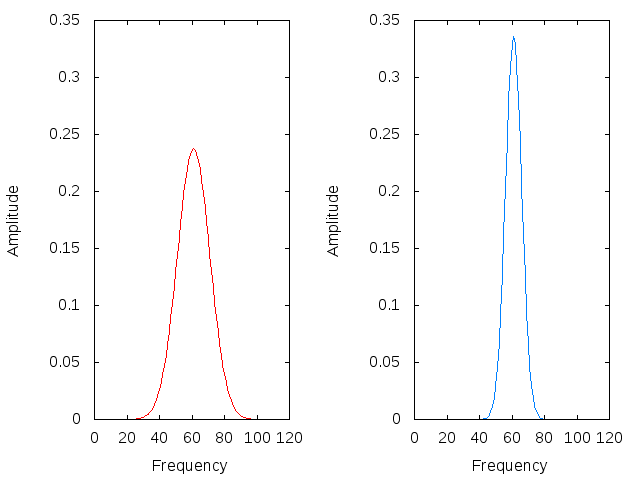
\includegraphics[width=1\textwidth]{single_sig_idler1.png}
        \caption{Signal (red) and Idler (blue)}
        \end{subfigure}
    \end{figure}

\end{frame} 

%slide 8
\begin{frame}{Non-separable JSAs} 
    \begin{figure}
        \centering
        \begin{subfigure}{0.45\textwidth}
            \movie[height=0.9\textwidth,width=1.1\textwidth, loop, autostart]{}{singlejsaentangledhermitegauss.mp4}
        \end{subfigure}
        ~
        \begin{subfigure}{0.45\textwidth}
        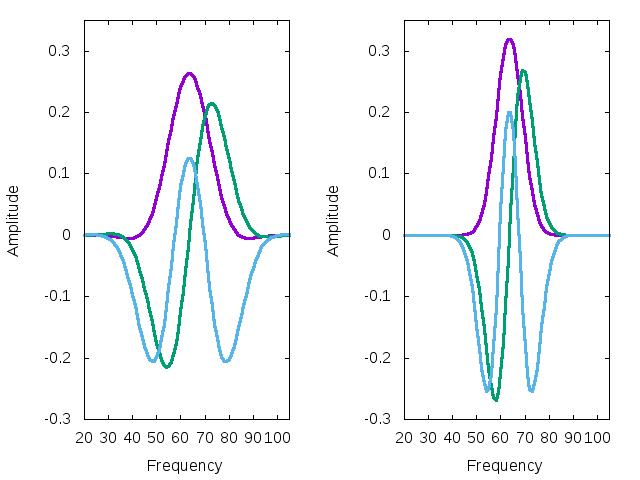
\includegraphics[width=1\textwidth]{singlesigidler_entangled_hermitegauss.png}
        \caption{Signal (red) and Idler (blue)}
        \end{subfigure}
    \end{figure}

\end{frame} 




%slide 9
\begin{frame}
\frametitle{Gaussian Optics}
\begin{itemize}
    \item Using the undelpeted pump approximation we can write the Hamiltonians as terms which are at most quadratic in creation and annihilation operators. 
    \item These are Gaussian transforms, they take Gaussian states to Gaussian states 

\end{itemize}
\begin{equation}
    \begin{bmatrix} 
        \vec{\b}   \\
        \vec{\bdag}
    \end{bmatrix}
    = 
    M
    \begin{bmatrix}
        \vec{\a} \\
        \vec{\adag}
    \end{bmatrix}
\end{equation}
\end{frame}



% slide 10
\begin{frame}
\frametitle{Types of Gaussian transformations}
%
\begin{figure}[h]
\begin{align*}
\centering
    \Qcircuit @C=0.6cm @R=0.2cm{
    %1
        &\lstick{a_1} &\qw &\multigate{1}{Squeezer} &\qw &\qw &\measureD{} \\
    %2
        &\lstick{a_2} &\qw &\ghost{Squeezer} &\qw  &\multigate{1}{BS} &\measureD{} \\
    %3
        &\lstick{a_3} &\qw &\multigate{1}{Squeezer} &\qw &\ghost{BS} &\measureD{} \\
    %4
        &\lstick{a_4} &\qw &\ghost{Squeezer} &\qw &\qw &\measureD{} \\
}
\end{align*}
\caption{Two source HOM dip}
\end{figure}
%
    \vspace{-20pt}
% 
\begin{figure}[h]
\begin{align*}
\centering
    \Qcircuit @C=0.5cm @R=0.2cm{
    %1
        &\lstick{a_1} &\qw &\multigate{1}{Squeezer} &\qw &\qw &\measureD{} & \\
    %2
        &\lstick{a_2} &\qw &\ghost{Squeezer} &\qw  &\multigate{1}{PBS} &\gate{\pi/4} &\measureD{H \& V} \\
    %3
        &\lstick{a_3} &\qw &\multigate{1}{Squeezer} &\qw &\ghost{PBS} &\measureD{} \\
    %4
        &\lstick{a_4} &\qw &\ghost{Squeezer} &\qw &\qw &\measureD{} \\
}
\end{align*}
\caption{Type-1 Fusion gate}
\end{figure}
%
\end{frame}

%slide 11
\begin{frame}{Two  squeezers JSA} 
    \begin{figure}
        \centering
        \begin{subfigure}{0.45\textwidth}
       \movie[height=0.9\textwidth, width=1\textwidth, loop, autostart]{}{jsa12pickme.mp4}
        \end{subfigure}
        ~
        \begin{subfigure}{0.45\textwidth}
        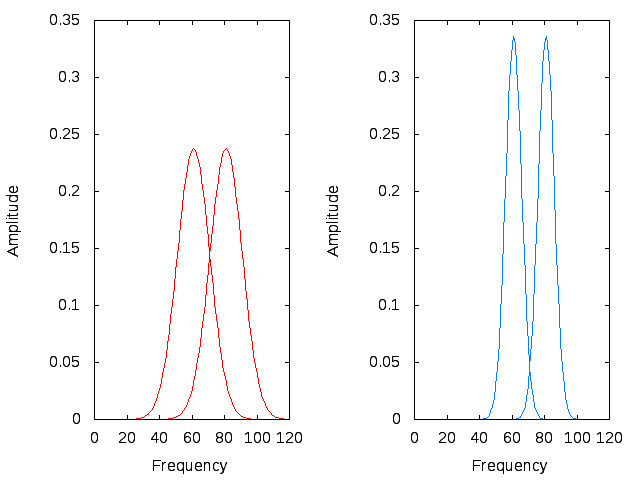
\includegraphics[width=1\textwidth]{single_sig_idler12.png}
    \end{subfigure}
   \end{figure}

\end{frame} 

% slide 12
\begin{frame}
    \frametitle{G(4) correlation function}
    \begin{equation}
        G^{(4)} = \frac{ \left< \creata_1 \creata_2 \creata_3 \creata_4 \annia_1 \annia_2 \annia_3 \annia_4 \right>}
        {\left< \creata_1 \annia_1 \right> \left< \creata_2 \annia_2 \right> \left< \creata_3 \annia_3 \right> \left< \creata_4 \annia_4 \right>}
    \end{equation}
  
    \begin{figure}[h]
       \movie[height=0.55\textwidth, width=1\textwidth, loop, autostart]{}{g4python.mp4}
    \end{figure}
    \begin{itemize}
	\item   
\end{itemize}
\end{frame}

%slide 13
\begin{frame}
\frametitle{Outlook}
\begin{itemize}
    \item There is much to do
\end{itemize}
\end{frame}

\end{document}
